\section{Présentation}
L'UMR MIA Paris-Saclay est une entité de recherche qui regroupe des
statisticiens et des informaticiens spécialisés dans la modélisation et
l'apprentissage statistique et informatique appliqués à la biologie, l'écologie,
l'environnement, l'agronomie et l'agro-alimentaire. Elle est affiliée à
AgroParisTech, INRAE et l'Université Paris Saclay.

Les membres de cette unité possèdent des compétences variées en matière de
méthodes d'inférence statistique, telles que les modèles complexes, les modèles
à variables latentes, l'inférence bayésienne, l'apprentissage et la sélection de
modèle. Ils sont également experts en algorithmique, notamment en
généralisation, transfert de domaine et représentation des connaissances.

L'objectif de cette unité est de développer des méthodes statistiques et
informatiques originales, à la fois génériques et motivées par des
problématiques spécifiques dans le domaine des sciences du vivant. Les activités
de recherche s'appuient sur une solide culture dans les disciplines cibles,
telles que l'écologie, l'environnement, l'agro-alimentaire, la biologie
moléculaire et la biologie des systèmes.

L'unité est structurée en deux équipes de recherche : SOLsTIS (Statistical
mOdelling and Learning for environnemenT and lIfe Sciences) et EkINocs (Expert
Knowledge, INteractive modellINg and learnINg for understandINg and decisiOn
makINg in dINamic Complexe Systems).

Elle est rattachée au département MATHNUM d'INRAE et au département MMIP
d'AgroParisTech.

Les responsables au sein de l'unité sont : Julien Chiquet en tant que Directeur
d'unité, Sophie Donnet en tant que Directrice d'unité adjointe, Antoine
Cornuéjols en tant que Responsable de l'équipe EkINocs, et Sophie Donnet
et Pierre Barbillon en tant que Responsables de l'équipe SOLsTIS.
\newline
\emph{Source:~\cite{AccueilMIAParisSaclay}}\\
La figure \ref{fig:organigramme-umr} présente l'organigramme complet de l'unité.

\begin{sidewaysfigure}[h!]
    \begin{center}
        % 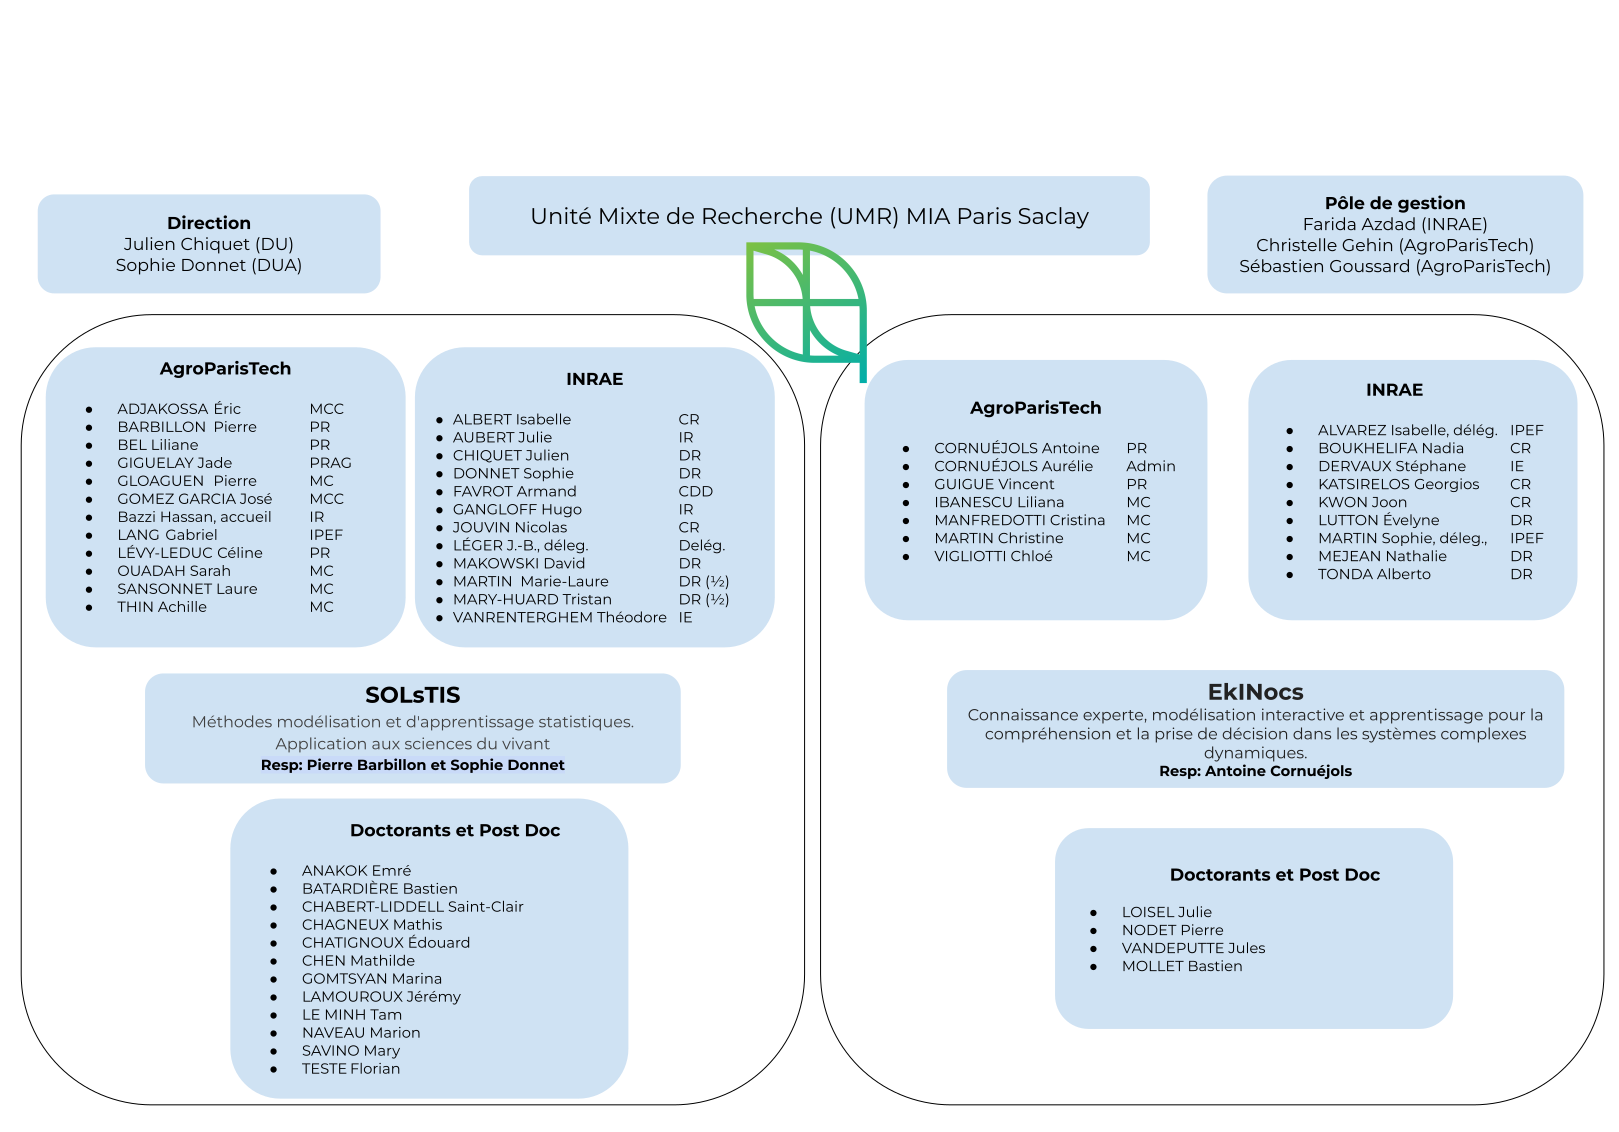
\includegraphics[scale=0.4]{img/Organigramme_MIA-Paris-Saclay}
        \includesvg[scale=0.6]{img/Organigramme_MIA-Paris-Saclay.svg}
        \caption{Organigramme de l'UMR}
        \label{fig:organigramme-umr}
    \end{center}
\end{sidewaysfigure}

\section{Encadrement et vie en stage}

Au cours de mon stage, j'étais encadré par Pierre Barbillon et fréquemment en
discussion avec lui et Saint-Clair Chabert-Liddell dont j'ai poursuivi les
travaux.

Le contexte de travail, au sein des ingénieurs d'études, des doctorants, des
chercheurs et des maîtres de conférences, a été pour moi très enrichissant. Ce
stage s'inscrit dans la construction de mon parcours professionnel en validant
le désir que je présentais de faire de la recherche.

Par ailleurs, divers projets entrepris au sein du laboratoire ont permis de
nouer des relations amicales en dehors des heures de travail. Par exemple, le
projet de construction d'une borne d'arcade pour le laboratoire, impulsé par
Julien Chiquet, a été une expérience extrêmement agréable et captivante à
laquelle prendre part.

J'ai particulièrement apprécié la disponibilité de toutes les personnes de
l'unité qui n'ont jamais hésité à se rendre disponible pour répondre à mes
questions.
Les nombreux séminaires et le désir de partage de connaissances à travers des
formations internes et de l'auto-formation m'a vraiment plu et m'a ouvert à de
nouvelles problématiques passionnantes.
De plus j'ai beaucoup progressé dans les domaines abordés pendant mon
stage, et cela m'a rendu confiant dans le choix de faire le
master \emph{MathSV} pour l'année scolaire 2023-2024. Ce stage a donc été
déterminant et confirme l'orientation de mon parcours professionnel.

\paragraph*{Note} La suite de ce rapport a été rédigée en anglais.